% CSE 5999 Progress Report #1 -- Brian Zhou
% IEEE CVPR 2023 template (camera-ready mode so the author is shown)
\documentclass[10pt,twocolumn,letterpaper]{article}

\usepackage[T1]{fontenc}   % so Times (the template font) also works under XeTeX/Tectonic
\usepackage[pagenumbers]{cvpr}

\usepackage{graphicx}
\usepackage{amsmath}
\usepackage{amssymb}
\usepackage{booktabs}
\usepackage{algorithm}
\usepackage{algpseudocode}
\usepackage[breaklinks,colorlinks]{hyperref}
\usepackage[capitalize]{cleveref}
\crefname{section}{Sec.}{Secs.}
\Crefname{section}{Section}{Sections}
\Crefname{table}{Table}{Tables}
\crefname{table}{Tab.}{Tabs.}
\crefname{algorithm}{Alg.}{Algs.}

\def\cvprPaperID{*****}
\def\confName{CSE 5999}
\def\confYear{2026}

\begin{document}

\title{Progress Report \#1: Learning Multi-Modal Travel Speed\\from Remote Sensing and GPS Traces}

\author{Brian Zhou\\
Washington University in St.\ Louis\\
{\tt\small zhou.n@wustl.edu}\\
{\small CSE 5999 Independent Study, Fall 2026 \;$\cdot$\; Mentors: Danni Beaulieu, Tianyi Gao \;$\cdot$\; Advisor: Prof.\ Nathan Jacobs}
}
\maketitle

%-----------------------------------------------------------------------------
\begin{abstract}
I am testing Tobler's 1993 hiking function against crowd-sourced GPS traces from OpenStreetMap (OSM) and asking whether remotely sensed terrain and vegetation structure can replace the trail attributes that maps usually lack. Since the plan, I ran the first go/no-go check (Gate~1) on real data: 6.47M GPS points in 12 boxes across three candidate regions. Gate~1 passes: 44--54\% of on-trail points are timestamped, and on-trail speeds fall in the walking range. However, the sample boxes contain only 54--82 hiking traces per region, far fewer than the plan assumed. Real data also exposed three bugs in my audit code, now fixed. A first, unvalidated fit suggests hikers are about 20--30\% slower than Tobler at the optimal slope and less sensitive to grade.
\end{abstract}

%-----------------------------------------------------------------------------
\section{Project Plan and Scope}
\label{sec:plan}

\paragraph{Problem.} Tobler's hiking function~\cite{tobler1993}, $v = 6\exp(-3.5\,|s+0.05|)$ (km/h, slope $s$ as rise/run), is still the default travel-speed model in GIS, yet it was fit to textbook figures rather than to observed movement. OSM sometimes records trail attributes such as \texttt{surface}, \texttt{sac\_scale} (difficulty) and \texttt{width} that should predict speed, but these tags are missing exactly where prediction matters most. My central question is: \emph{can remotely sensed terrain and vegetation structure substitute for trail attributes that a map does not have?} The experiment is a four-arm comparison in which every arm predicts segment speed and the arms differ only in their inputs: \emph{Tobler} (slope, fixed coefficients), \emph{Tags} (OSM attributes + slope), \emph{Remote sensing} (LiDAR/imagery covariates + slope, no tags), and \emph{Both}.

\paragraph{Goals.} My \emph{minimum} goal, which I am confident I can reach, is a cleaned, stop-filtered, map-matched trajectory dataset for one high-relief forested region, joined to 1\,m terrain and vegetation covariates, together with the empirical slope--speed curve and an honest comparison against Tobler. My \emph{maximum} goal is the full four-arm comparison with heteroscedastic models that predict speed and its uncertainty, directional asymmetry measured on out-and-back hikes, and per-mode curves, written up as a four-page IGARSS 2027 paper (deadline 11 January 2027) entered in the Student Paper Competition.

\paragraph{Scope changes since the project plan.}
(i)~\emph{Dataset scale.} Gate~1 shows the OSM trace supply is hundreds of hikes per region, not the tens of thousands anticipated (\cref{sec:results}). The design is unchanged, but model capacity must match: a parametric Tobler-form backbone, a regularized boosted-tree baseline, and possibly two pooled regions (which also allows a geographic hold-out).
(ii)~\emph{Travel mode.} If the White Mountains is chosen, the bikes-vs.-walkers question becomes a stated limitation, because 86\% of on-trail time there is on foot-only trails.
(iii)~\emph{New baseline.} I propose adding STRIDE~\cite{campbell2024stride} as a second closed-form baseline next to Tobler (\cref{sec:related}).
(iv)~\emph{Schedule.} I ran Gate~1 in week~6 rather than week~3. Following the plan's rule of slipping the back rather than the gates, I now target a full draft by mid-December.

%-----------------------------------------------------------------------------
\section{Related Work Update}
\label{sec:related}

\paragraph{Speed from overhead imagery (Jacobs group).}
RasterNet~\cite{hadzic2020rasternet} fuses aerial imagery and airborne LiDAR in a geospatially consistent raster to regress road free-flow speed without hand-measured road geometry. I keep its premise (regress speed from overhead data when curated attributes are missing) but move it to trails, where slope dominates and supervision comes from noisy crowd-sourced traces. Its raster alignment is my reference design for the covariate stack.
Workman and Jacobs~\cite{workman2020dynamic} (CVPR 2020) condition a CNN on overhead imagery, location and time to output a local motion model of travel directions and speeds. Its explicit treatment of \emph{direction} parallels my need for signed, direction-aware slope.
Workman and Hadzic~\cite{workman2024probabilistic} (ECCV 2024) predict \emph{distributions} of traffic speed from imagery with a probabilistic objective. This supports my plan to predict speed variance and evaluate with proper scoring rules~\cite{gneiting2007strictly} rather than reporting point error alone.

\paragraph{Pedestrian travel rates.}
HikingTTE~\cite{asako2024hikingtte} estimates hiking time with an LSTM, attention, and an embedded modified-Lorentz slope--speed curve, personalized per hiker. It uses trajectories only, with no remote sensing, and its idea of a known curve inside a learned model matches my proposed backbone (\cref{sec:approach}).
Campbell \etal~\cite{campbell2022variability} use crowd-sourced GPS hikes to predict \emph{percentiles} of travel rate, showing that the spread between hikers is large and worth modeling. That motivates my heteroscedastic heads.

\paragraph{New since the plan: LiDAR-based travel rates.}
I found two papers from the same group that sit closest to my Question~2. STRIDE~\cite{campbell2024stride} is a single closed-form function of LiDAR-derived slope, vegetation density, and surface roughness that predicts on- \emph{and} off-path walking rates. It explains over 80\% of the variance in mean rates from three field experiments. Cutler \etal~\cite{cutler2026machine} fit a random forest to LiDAR slope, vegetation, and roughness for off-trail travel ($R^2 = 0.78$), with vegetation density the second most important factor.
STRIDE is calibrated on dedicated field experiments, and neither paper compares against OSM trail tags. My contribution is therefore (a)~supervision from many crowd-sourced hikes on real trails, (b)~a head-to-head test of remote sensing against OSM tags, and (c)~calibrated uncertainty. STRIDE also gives a stronger closed-form baseline than Tobler.
For the vegetation covariates, Campbell \etal~\cite{campbell2018understory} show that understory return density normalized by the pulse energy reaching each stratum is far more predictive than raw density. For the trace pipeline, I will follow HMM map-matching~\cite{newson2009hidden}.

%-----------------------------------------------------------------------------
\section{Proposed Approach}
\label{sec:approach}

\begin{algorithm}[t]
\caption{T1 trajectory pipeline for one region.}
\label{alg:t1}
\begin{algorithmic}[1]
\small
\For{each $0.25^\circ$ tile $b$ of the region}
  \State read OSM trackpoint pages $0,1,\dots$ until untimed points appear
  \State find last page by doubling + bisection; count untimed pts
  \State fetch the full GPX of each identifiable trace
\EndFor
\For{each trace and recording segment}
  \State drop repeated timestamps, $>$60\,km/h steps, $>$5\,min gaps
  \State flag stops (speed + minimum-duration rule)
  \State HMM map-match to OSM trails~\cite{newson2009hidden}; drop low-confidence matches
  \State resample matched path into $L$\,m segments, $L\!\in\!\{25,50\}$
  \State store length, time, speed, signed slope, tags, interval, date
\EndFor
\State remove duplicate uploads; label outings, uploaders, trail systems
\end{algorithmic}
\end{algorithm}

\paragraph{T1: trajectory dataset (\cref{alg:t1}).}
I tile the chosen region into $0.25^\circ$ boxes, the API maximum (about 12 for the White Mountains), and query \nolinkurl{api.openstreetmap.org/api/0.6/trackpoints}. The API returns every timestamped point first (newest upload first), then untimed points sorted by latitude. Reading until untimed points appear and then bisecting for the last page counts the unusable points exactly from about a dozen of their pages. Every response is cached. For identifiable traces I fetch the original GPX (\nolinkurl{openstreetmap.org/trace/<id>/data}), giving whole hikes rather than box-clipped pieces. Cleaning per recording segment is already implemented. I will tune the stop rule on about 20 hand-labeled stops and report the time removed. Map-matching will use \texttt{leuvenmapmatching}, an HMM matcher, on a trail graph built with \texttt{pyrosm} from a Geofabrik extract (sidewalks excluded), and I will report the match rate. Slope is signed along the direction of travel and checked by a unit test.

\paragraph{T2: remote sensing covariates.}
From the USGS 3DEP 1\,m DEM I will derive slope, aspect, curvature, roughness and TPI with \texttt{gdaldem} and the Relief Visualization Toolbox. Vegetation structure comes from USGS point clouds, streamed with PDAL from the public \texttt{usgs-lidar-public} Entwine bucket within a 30\,m buffer of traced trails. The metric is normalized return density in the 0.5--1.5, 1.5--2.5 and 2.5--3.5\,m strata~\cite{campbell2018understory}. I will add NLCD canopy cover, NAIP spectral indices and point-sampled AlphaEarth embeddings through Earth Engine, aligned on a common raster following RasterNet~\cite{hadzic2020rasternet}.

\paragraph{T3: models and evaluation.}
The backbone keeps Tobler's form but lets its constants depend on covariates $\mathbf{x}$:
\begin{equation}
\log v = \log v_0(\mathbf{x}) - k(\mathbf{x})\,|s + s_0(\mathbf{x})| + \varepsilon,
\end{equation}
where $\varepsilon$ follows a Student-$t$ distribution with a scale predicted per segment (the heteroscedastic head), plus a partially pooled per-hiker offset. Each arm feeds its allowed covariates to small heads for $v_0$, $k$ and $s_0$, so the fitted parameters stay interpretable (\eg, ``$k$ is lower under dense understory''). Baselines are Tobler, STRIDE, and LightGBM with a monotone constraint on uphill grade. Before any model, I will run the log-linear diagnostic: under Tobler, $\log v$ against $|s+0.05|$ is a straight line of slope $-3.5$. Metrics are MAE/RMSE on segment speed, NLL and CRPS~\cite{gneiting2007strictly}, and PIT histograms. Splits are by trace and by trail system, never by point.

%-----------------------------------------------------------------------------
\section{Data and Resources}
\label{sec:data}

\paragraph{GPS traces.} OSM GPX traces, retrieved through the URL above at 5{,}000 points per page. Uploaders choose a visibility level. \emph{Identifiable} and \emph{trackable} traces keep ordered timestamps and are usable. \emph{Public} and \emph{private} points come back untimed and sorted by position, so they are unusable for speed. A real record from one hike (\cref{fig:example}) looks like this:
{\small\begin{verbatim}
<trkpt lat="44.2576116" lon="-71.2520930">
  <time>2013-07-04T11:20:07Z</time></trkpt>
\end{verbatim}}
\noindent The trace contains 4{,}813 such points recorded every $\sim$7\,s over 10\,h: a 17\,km loop from Pinkham Notch toward Mt Washington, with a median moving speed of 2.0\,km/h and 26\% of its time stopped. The Gate~1 sample holds 6.47M points (5.19M timestamped) in 12 boxes of $0.1^\circ\!\times\!0.1^\circ$, four per region: 1{,}707 usable traces, 216 of them hiking traces (630 trail-hours), and 0.6\,GB of cache. There are \emph{no ground-truth annotations}. Speed comes from timestamps, mode will be inferred, and OSM tags are attributes.

\begin{figure}[t]
\centering
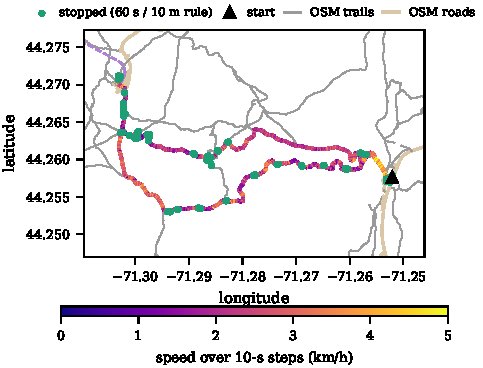
\includegraphics[width=\linewidth]{figures/fig_example_trace.pdf}
\caption{Actual data: one trackable OSM trace (4{,}813 points, 4 July 2013) on the OSM trail network near Mt Washington, colored by speed over 10\,s steps. Green dots mark stops found by the duration rule.}
\label{fig:example}
\end{figure}

{\raggedright\paragraph{Trail graph and tags.} OSM ways come from Overpass for Gate~1 and from Geofabrik extracts for T1. A real example way: \texttt{highway=path}, \texttt{name=Gulfside Trail}, \texttt{sac\_scale=mountain\_hiking}, \texttt{surface=ground}, \texttt{bicycle=no}, \texttt{horse=no}. Tag coverage is incomplete: in the White Mountains boxes, \texttt{surface} is present on 58\% of trail length, \texttt{sac\_scale} on 40\%, and \texttt{width} on almost none.\par}

\paragraph{Remote sensing.} USGS 3DEP 1\,m DEMs, the 3DEP work-unit index (quality level, dates), 3DEP point clouds on AWS, NLCD 2021 tree canopy (MRLC), and NAIP and AlphaEarth via Earth Engine.

\paragraph{Platform.} Python 3.12 (numpy, pandas, scipy, matplotlib) on my laptop (Apple M4, 16\,GB) for T1 and T3. For T2's point clouds I will use the McKelvey Engineering compute cluster, whose project storage already holds the lab's OSM data.

%-----------------------------------------------------------------------------
\section{Results So Far}
\label{sec:results}

\begin{table}[t]
\centering
\footnotesize
\setlength{\tabcolsep}{2pt}
\begin{tabular}{@{}lccc@{}}
\toprule
 & White Mtns & Cascades & Front Range \\
\midrule
GPS points (4 boxes) & 0.54M & 1.46M & 4.48M \\
Usable: all / on-trail points & 58 / 46\% & 82 / 44\% & 82 / 54\% \\
Hiking traces (outings) & 54 (51) & 80 (77) & 82 (82) \\
Named users + anon.\ traces & 17 + 26 & 25 + 34 & 19 + 20 \\
Trail-hours; median speed & 254\,h; 2.7 & 191\,h; 3.2 & 185\,h; 4.1 \\
Foot-only trail time & 86\% & 69\% & 36\% \\
Cyclist-speed traces & 0 & 4 & 7 \\
1\,m DEM: boxes / region & 100 / 100\% & 56 / 70\% & 98 / 100\% \\
Best LiDAR QL (years) & QL2 (15--18) & QL1 (16--21) & QL1 (20--23) \\
NLCD tree canopy & 79\% & 46\% & 23\% \\
\texttt{sac\_scale} on trails & 40\% & 55\% & 24\% \\
Stops removed: 0.5\,km/h / 60\,s & 20 / 24\% & 19 / 21\% & 13 / 15\% \\
\bottomrule
\end{tabular}
\caption{Gate~1 on real OSM data (4 sample boxes per region). ``On-trail'' means within 25\,m of an OSM path, not a sidewalk. Hiking traces have $\geq$5 moving minutes on trails. Speeds are in km/h.}
\label{tab:gate1}
\end{table}

\paragraph{Implemented.} (1)~The Gate~1 audit: paged download with exact counts, caching, per-segment cleaning, nearest-way matching (trails vs.\ roads, lifts, sidewalks), two stop rules, and summaries. (2)~A region-layer audit (1\,m coverage, LiDAR quality, relief, canopy). (3)~A first slope--speed look. A 29-check fake-data self-test passes. Not yet: the full-region download, HMM map-matching, fixed-length segments, T2, T3.

\paragraph{Gate~1 outcome (\cref{tab:gate1}).} Gate~1 passes: 44--54\% of on-trail points are usable, median on-trail speeds of 2.7--4.1\,km/h lie in the walking range, and the Front Range and Cascades show a faster cyclist mode. The binding constraint is \emph{volume}: 54--82 hiking traces per region in the samples, from at most 39--59 distinct uploaders (named users plus anonymous traces), with one uploader contributing 23 Front Range traces. A full region may yield a few hundred hikes. Also: driver-assistance car loggers (sunnypilot/dragonpilot) make up most ``identifiable'' uploads in two regions, hence the on-trail metric. Two stop rules remove 13--24\% of trail time but disagree on which minutes. GPS jitter inflates speed only 2--3\% on real 1--2\,s data ($n{=}43$). The Rainier box has no 1\,m DEM.

\paragraph{Bugs found on real data.} Three errors surfaced once my synthetic-tested audit code met real data. First, because usable points arrive first, a 10-page cap reported $\sim$100\% usable where the truth is 60\% (Mt Washington box). Second, uploads holding several out-of-order recordings were misread as shuffled. Third, 10\,Hz car loggers with whole-second timestamps were read at walking pace. All three are fixed and covered by the self-test.

\begin{figure}[t]
\centering
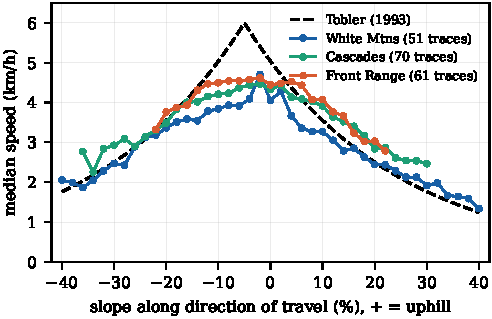
\includegraphics[width=\linewidth]{figures/fig_slope_speed.pdf}
\caption{First look (not validated): median speed per 2\% slope bin from 23{,}302 on-trail chunks of $\sim$50\,m (182 walker traces), with elevation from a 5\,m USGS DEM. Fitted $(v_0,k)$: White Mtns (4.3, 2.2), Cascades (4.6, 1.6), Front Range (4.9, 1.8), against Tobler's (6.0, 3.5).}
\label{fig:slope}
\end{figure}

\paragraph{First look at slope vs.\ speed (\cref{fig:slope}).} Fitting $\log v = \log v_0 - k|s+s_0|$ to walkers gives a fastest slope of $-4$ to $-5.5\%$, in agreement with Tobler's $-5\%$. However, $v_0$ is 19--28\% lower and $k$ is 38--54\% lower: hikers are slower on gentle grades and closer to Tobler on steep ones. The White Mountains curve is the slowest at nearly every slope, which is the kind of regional difference terrain and vegetation covariates should explain. Caveat: slope noise also flattens fitted curves, so this waits on T1's clean segments.

%-----------------------------------------------------------------------------
\section{External Assistance and Collaboration}
\label{sec:help}

My PhD mentors, Danni Beaulieu and Tianyi Gao, guide the project in weekly meetings. Danni scoped the semester plan (its gates, four-arm design and candidate regions) and shared the lab's existing OSM data with me. Prof.\ Nathan Jacobs is my faculty advisor. At Danni's suggestion I use Claude (Anthropic), an AI assistant. It wrote the first version of my reading notes and audit code; tested, debugged and rewrote the Gate~1 and region-audit scripts; ran the downloads and analyses; checked data-service behavior; and helped draft this report. I reviewed the code, results and text and am responsible for them. Data come from OSM contributors, USGS 3DEP and MRLC.

%-----------------------------------------------------------------------------
\section{Reservations and Questions}
\label{sec:questions}

\begin{itemize}\setlength\itemsep{1pt}
\item \textbf{Is the volume enough?} Samples hold only tens of independent hikers per region. Are a few hundred hikes enough, or should I pool regions or add sources?
\item \textbf{Region choice.} The White Mountains have the most forest, full 1\,m coverage and trail-hours, but are foot-only with QL2 LiDAR. The Cascades I-90 corridor has QL1 LiDAR and more tags but fewer hours.
\item \textbf{Hardest steps.} Stop detection and map-matching under canopy (to be validated by hand), slope noise biasing $k$ toward zero, and season (36\% of White Mountains trail time is winter).
\item \textbf{Positioning} against STRIDE and Cutler \etal, and whether STRIDE should be a baseline arm.
\item \textbf{Access.} I have lab swipe access, and the lab's OSM data is on the cluster's ENGRFS storage. Next: inspect it (does it cover part of T1?) and set up Earth Engine before T2 (about week~10).
\end{itemize}

{\footnotesize
\setlength{\itemsep}{0pt}\setlength{\parskip}{0pt}
\bibliographystyle{ieee_fullname}
\bibliography{refs}
}

\end{document}
